\section{Benchmark and identification protocol}\label{sec:bench}

\subsection{Levels of the benchmark}\label{sec:levels}

The benchmark is designed to separate two properties, hiddenness and rarity, and to test the method on all types of systems for which heuristics have been proposed. Equations, parameters, and integration settings are given in Appendix~\ref{app:systems}, and a summary is given in Table~\ref{tab:benchmark}. A gallery of level-A attractors is shown in Fig.~\ref{fig:gallery3d}.
\begin{itemize}
\item \textbf{Level A: three-dimensional flows.} The Chua circuit with two parameter sets\cite{Leonov2011PLA,GuanXie2025,Kuznetsov2023Chua} (Fig.~\ref{fig:chuaII} and Appendix~\ref{app:systems}). Systems without equilibria: NE4, Wang--Chen \#1, and Wei,\cite{Wei2011,JafariSprottGolpayegani2013} as well as the 2026 system of Jafari \textit{et al.} without fixed and perpetual points.\cite{Jafari2026NoPP} Systems with a single stable equilibrium: Wang--Chen \#2, SE3, and SE11.\cite{WangChen2012,Molaie2013} The LE1 system with a line of equilibria\cite{JafariSprott2013} and the Rabinovich system.\cite{Kuznetsov2018Rabinovich} The negative controls are the transient chaos of the Lorenz system at $(a,r,b)=(4,29,2)$\cite{YorkeYorke1979} and the ``hidden attractor'' of the Rabinovich system at $r=6.8$, which, according to Ref.~\onlinecite{SprottMunmuangsaen2018Comment}, is a transient set.
\item \textbf{Level B: maps.} The map of Huynh \textit{et al.} without fixed points.\cite{Huynh2019} Eight cases of the general family of Jiang \textit{et al.}:\cite{Jiang2016Maps} four without fixed points and four with a single stable one. Three parameter sets of the same family in the form of Ref.~\onlinecite{Ouannas2018}. The H\'enon map serves as a control. Phase--basin portraits of the maps and of the other systems are given in Appendix~\ref{app:systems}.
\item \textbf{Level C: four-dimensional systems.} The simplified Lorenz system of Li and Sprott without equilibria\cite{LiSprott2014} in three regimes (a torus and a pair of strange attractors; a cycle and a pair; hyperchaos) and the system of Jahanshahi \textit{et al.}\cite{Jahanshahi2019} This level is used for the census and the verification protocol; the search experiments are run on levels A, B, and D.
\item \textbf{Level D: synthetic families} with analytically known basin measure (Sec.~\ref{sec:synth}).
\end{itemize}

The region $B$ for three-dimensional systems is the cube $[-10,10]^3$, the natural region of the original publications. For the Chua circuit, we take the box $[-10,10]^2\times[-15,15]$ proposed in Ref.~\onlinecite{Zelinka2016}. For NE4 and the Rabinovich system, the region is twice the extent of the attractor. Basin fractions are estimated from $5\times10^4$ uniform points for level A and $2\times10^4$ for the other levels; for the Chua circuit, they were checked by an independent computation in Attractors.jl.\cite{Datseris2018JOSS,DatserisWagemakers2022}

Table~\ref{tab:benchmark} confirms that hiddenness and rarity are different properties. In the Rabinovich system and in Wang--Chen \#2, the hidden attractor occupies 76\% and 67\% of the region. Only the targets of Chua~II, SE11, LE1, the Jafari cycle and chaos, and the Huynh map are rare ($p<10^{-2}$). The Jiang maps, which Ref.~\onlinecite{Jiang2016Maps} characterizes as having ``tiny'' basins, give $p\approx0.03$--$0.10$ in boxes around the attractor. The classical heuristics behave on this benchmark as described in the review in Ref.~\onlinecite{GuanXie2025}, and none of them helps on the rare targets (Appendix~\ref{app:classic}). The literature baseline for the search experiments is differential evolution (DE) over initial conditions with the cost function of Ref.~\onlinecite{Zelinka2016}, which, unlike our strategies, is given the size of the target (Appendix~\ref{app:ablation}).

\begin{table*}
\caption{Benchmark: search targets (hidden attractors), basin measures $p$ in the region $B$, and the cost of uniform sampling $N^0_{0.9}$. Basin measures are from the uniform census ($5\times10^4$ points for level A, $2\times10^4$ otherwise); $N^0_{0.9}$ is the 0.9 quantile of the first-hit index over $R=50$ runs of uniform sampling ($R=20$ for the Jafari chaos; for the nonrare targets, it is $\lceil\ln0.1/\ln(1-p)\rceil$). A slash separates two symmetric attractors, a semicolon separates different targets, and ``both'' means the cost of hitting either of the two; the search tables of Sec.~\ref{sec:results} use the combined measure of the two symmetric attractors and remeasure $N^0_{0.9}$ with their own runs. $\lambda$ is the largest Lyapunov exponent.}
\label{tab:benchmark}
\footnotesize
\setlength{\tabcolsep}{4pt}
\begin{ruledtabular}
\begin{tabular}{llllrr}
Level & System & Equilibria & Target & $p$ & $N^0_{0.9}$ \\
\hline
A & Chua I & F$_0$ stable, F$_\pm$ saddle-foci & two chaotic (A, B) & 0.017 / 0.018 & 136 / 124 \\
 & Chua II & F$_0$ saddle-focus, F$_\pm$ stable & cycle LC; two chaotic & 0.992; 0.0014 / 0.0013 & 1; 772 (both) \\
 & NE4 & none & chaos ($\lambda\approx0.03$) & 0.33 & 6 \\
 & Wang--Chen \#1 & none & chaos & 0.103 & 22 \\
 & Wei (NE2) & none & chaos & 0.096 & 23 \\
 & Jafari 2026, $a_3=-1$ & none; no perpetual points & cycle & 0.009 & 229 \\
 & Jafari 2026, $a_3=-3.548$ & none & fragile chaos ($\lambda\approx0.05$) & $(2$--$5)\times10^{-4}$ & 5331 \\
 & Wang--Chen \#2 & one, stable & chaos & 0.666 & 3 \\
 & SE3 & one, stable & chaos & 0.153 & 14 \\
 & SE11 & one, stable & chaos & 0.0079 & 302 \\
 & LE1 & line $x=y=0$ & chaos & 0.0016 & 1422 \\
 & Rabinovich, $r=100$ & saddle at 0, two stable foci & chaos & 0.763 & 2 \\
\hline
B & Huynh 2019 & none & chaos & 0.0091 & 211 \\
 & Jiang 2016, NF I e, f, g, i & none & chaos & 0.028--0.039 & 59--82 \\
 & Jiang 2016, SF I a--d & one, stable & chaos & 0.065--0.10 & 22--37 \\
\hline
C & Li--Sprott 4D, $a=6$ & none & torus; two strange & 0.090; 0.446 / 0.464 & 25; 4 \\
\hline
D & D1, D2 (base SE3), $n=4$--14 & as for the base & chaos of the base & $10^{-2}$--$10^{-7}$ & 258--$2.1\times10^{7}$ \\
\end{tabular}
\end{ruledtabular}
\end{table*}

\begin{figure*}
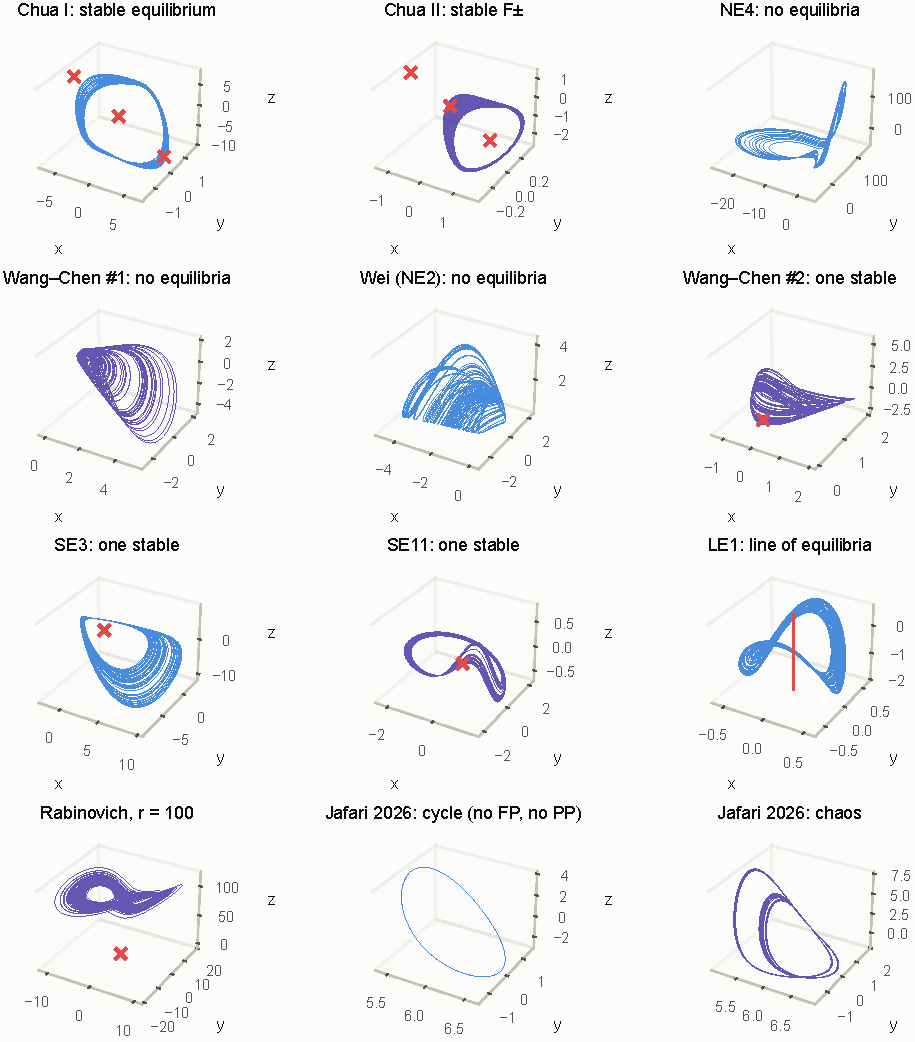
\includegraphics[width=\textwidth]{figures/fig32_gallery_3d.pdf}
\caption{Hidden attractors of the level-A benchmark. Crosses mark equilibria; for LE1, the red line is the line of equilibria $x=y=0$. NE4, Wang--Chen \#1, Wei, and the Jafari 2026 system have no equilibria, and in Wang--Chen \#2, SE3, and SE11 the single equilibrium is stable, so all attractors shown are hidden by definition.}
\label{fig:gallery3d}
\end{figure*}

\begin{figure*}
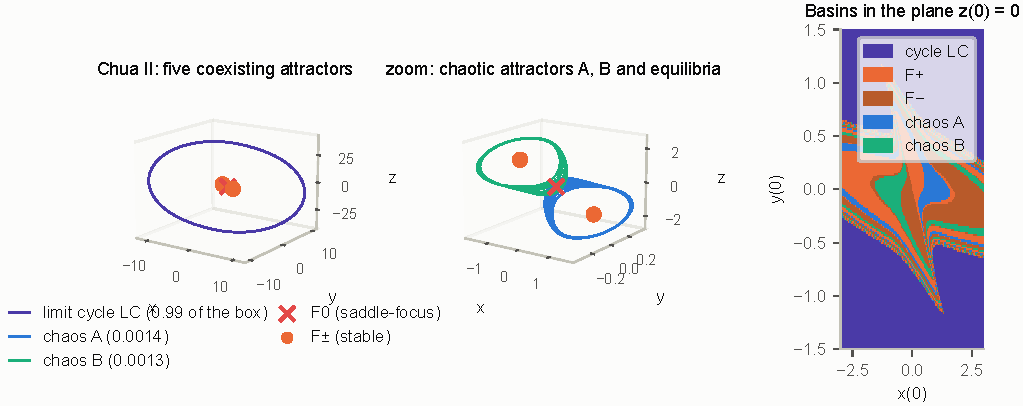
\includegraphics[width=\textwidth]{figures/fig31_chua_II_coexisting.pdf}
\caption{Chua circuit, parameter set II: five coexisting attractors. (a) The large limit cycle LC (basin fraction in the box 0.992), the chaotic attractors A and B (0.0014 and 0.0013), the saddle-focus F$_0$, and the stable foci F$_\pm$. (b) Enlarged fragment; the chaotic attractors surround F$_\pm$. (c) Basins in the plane $z(0)=0$ (window $|x|\le3$, $|y|\le1.5$, axes not to scale). The basins of the chaotic attractors are narrow strips between the basins of F$_\pm$ and of the cycle; a search can exploit only these boundaries and the long transients near them.}
\label{fig:chuaII}
\end{figure*}

\subsection{Synthetic families with known basin measure}\label{sec:synth}

To measure the scaling of the cost for $p$ down to $10^{-7}$ and dimensions up to 14, the three-dimensional system SE3 with a hidden attractor ($p_W=0.153$ in $[-10,10]^3$, where $W_{\rm HA}$ denotes its basin) is embedded in $\mathbb{R}^{3+m}$. The search region is $B=[-10,10]^3\times[-1,1]^m$. We use two constructions with opposite properties: D1 has no transient signal, and D2 has a signal on all scales.

\textbf{D1, ``embedding with a gate.''} The system is
\begin{equation}
\begin{split}
&\dot x=F(x)-g(w)\,(x-e),\qquad \dot w=-\kappa w,\\
&g(w)=\frac{H}{1+\exp\bigl(-400(|w|-\rho)/\rho\bigr)},
\end{split}
\label{eq:d1}
\end{equation}
where $e$ is the stable equilibrium of the base, $H=50$, and $\kappa=0.5$. While $|w|>\rho$, the ``gate'' pulls $x$ toward $e$. Therefore, the basin of the hidden attractor is approximately $W_{\rm HA}\times\{|w_0|\le\rho\}$, and
\begin{equation}
p(\rho,m)=p_W\,\frac{V_m(\rho)}{2^m},\qquad V_m(\rho)=\frac{\pi^{m/2}\rho^m}{\Gamma(m/2+1)}.
\label{eq:pD}
\end{equation}
The measured fractions agree with Eq.~\eqref{eq:pD} within 5\%--15\%. Outside a thin rim of the ball, the transient hardly depends on $|w_0|$, so channel B is practically absent in D1.

\textbf{D2, ``edge state.''} Here, the embedding is decoupled:
\begin{equation}
\dot x=F(x),\qquad \dot w=\kappa\, w\,\bigl(|w|^2/\rho^2-1\bigr),\qquad \kappa=1.
\label{eq:d2}
\end{equation}
The sphere $|w|=\rho$ is repelling. For $|w_0|<\rho$, the coordinates $w$ decay and $x$ follows the base; for $|w_0|>\rho$, the norm $|w|$ blows up in finite time. The target basin is exactly $W_{\rm HA}\times\{|w_0|<\rho\}$, and formula~\eqref{eq:pD} is exact given $p_W$; a check gave $p_{\rm meas}=0.00102$ and $0.00100$ at $p=0.001$. The escape time for $|w_0|=\rho(1+\Delta)$ equals $\ln\bigl((1+\Delta)^2/((1+\Delta)^2-1)\bigr)/(2\kappa)\approx\ln(1/2\Delta)/(2\kappa)$ for small $\Delta$. It diverges at the basin boundary (Fig.~\ref{fig:d2mech}), as for edge states of real systems.\cite{Vollmer2009Edge,LucariniBodai2017} In D2, channel B is informative on all scales down to the integration step.

\begin{figure*}
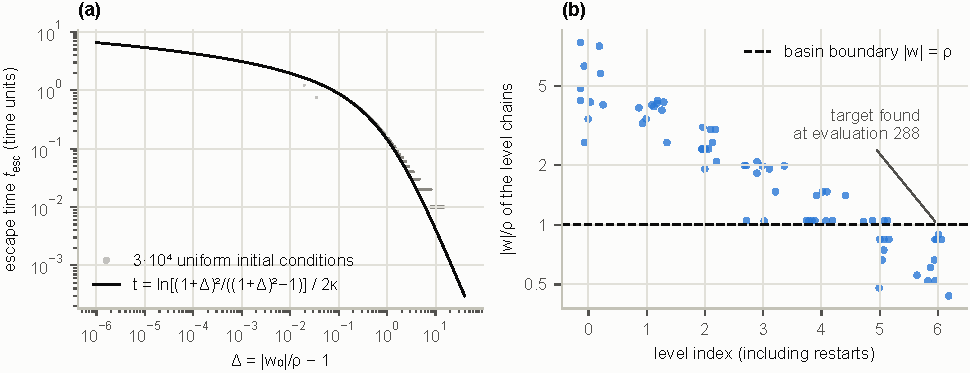
\includegraphics[width=\textwidth]{figures/fig37_d2_mechanism.pdf}
\caption{Mechanism of the splitting gain in family D2 ($n=6$, $p=10^{-4}$). (a) Escape time versus the relative distance to the basin boundary $\Delta=|w_0|/\rho-1$; dots are $3\times10^4$ uniform initial conditions, and the line is the exact law $\ln\bigl((1+\Delta)^2/((1+\Delta)^2-1)\bigr)/(2\kappa)$. The steps on the right reflect the discreteness of the integration step. (b) $|w|/\rho$ for the seeds of the chains over the levels of one run; the chains contract to the ball $|w|<\rho$, and the target is found after 288 integrations, whereas uniform sampling needs $N^0_{0.9}=1.7\times10^4$.}
\label{fig:d2mech}
\end{figure*}

\subsection{Identification and verification protocol}\label{sec:protocol}

\textbf{Trajectory fingerprint.} A trajectory is integrated by the fourth-order Runge--Kutta method (RK4) with a fixed step (maps are iterated) over the transient segment $T_{\rm tr}$ and the observation window $T_{\rm obs}$. Escape is detected by the condition $|x|>R_{\rm esc}$. On the observation window, we compute the largest Lyapunov exponent $\lambda$ by the two-trajectory method,\cite{Benettin1980} the mean speed, the maximum norm, the frequency of local maxima, the amplitude contraction ratio, and the coordinate-wise mean, standard deviation, minimum, and maximum. The same statistics are computed on an early window; they are needed by the reaction coordinate (Sec.~\ref{sec:xi}). The kernels are implemented in Numba\cite{Lam2015Numba} and compute the fingerprints inside the integrator, at about $3\times10^8$ RK4 steps per second on 14 cores.

\textbf{Templates and matching.} The template of a regime is the mean $\mu$ and spread $\sigma$ of the fingerprint over 64 copies. The copies start from random points of a trajectory segment on the attractor of length $4T_{\rm obs}$ (phase randomization) with relative noise $10^{-3}$. A trajectory with fingerprint $f$ is assigned to the template with the smallest
\begin{equation}
z=\max_i\frac{|f_i-\mu_i|}{\sigma_i+0.02\,(1+|\mu_i|)},
\label{eq:z}
\end{equation}
provided that $z<6$ and the classes are compatible: a chaotic template requires $\lambda>0.005$, and a regular one requires $\lambda<0.02$; in the overlap, the fingerprint decides. Converged trajectories are compared with equilibria by their final point with tolerance $10^{-3}L$, where $L$ is half the largest edge of $B$. Decaying trajectories ($\lambda<-0.002$ and amplitude contraction) are compared by the center of the window. Unmatched trajectories are clustered (DBSCAN), and a new template is calibrated for each cluster; this is how unknown regimes are discovered, during a search as well as in the enumeration of the regimes of a new system.

\textbf{Verification.} Each candidate passes four checks: the lifetime (the integration is continued for at least 20 windows and, for claims of a chaotic attractor, up to $10^4$--$10^5$ time units), convergence in the step (the same template and stable basin fractions under $\Delta t\to\Delta t/2$), an independent integrator (DOP853\cite{Hairer1993} with $\mathrm{rtol}=10^{-11}$ and Attractors.jl with Vern9), and the sign of the Lyapunov exponent over consecutive windows. For claims of hiddenness, $h_\varepsilon$ is estimated by sampling in the $\varepsilon$-neighborhoods of all equilibria and along their unstable manifolds, $\varepsilon\in\{10^{-3},10^{-2},10^{-1}\}L$; it distinguishes deeply hidden attractors (SE3, SE11) from shallowly hidden ones (Chua~I, the Rabinovich system), and the number of starts bounds its resolution (Appendix~\ref{app:verification}). The protocol was refined on three cases that change the conclusions if missed (Appendix~\ref{app:verification}): a numerical ``transient chaos'' of the Chua circuit at $\Delta t=0.01$, which underestimates the fractions of the hidden attractors almost twofold; a published table of basin fractions whose hidden-attractor fractions coincide with ours only at that coarse step; and intermittency and long-lived transient sets mistaken for attractors. The step-convergence and lifetime checks are therefore mandatory.
